\documentclass[12pt,a4paper]{article}
\usepackage{a4wide}
\usepackage[utf8]{inputenc}
\usepackage[greek,english]{babel}
\usepackage{alphabeta}
\usepackage{array}
\usepackage{mathtools}
\usepackage{ragged2e}
\usepackage{graphicx}
\graphicspath{ {./images/} }
\usepackage[top=60pt,bottom=55pt,left=55pt,right=55pt]{geometry}

\title{Αλγόριθμοι και Πολυπλοκότητα \\* 2η Σειρά Ασκήσεων}
\author{ Καραβαγγέλης Αθανάσιος \\ Α.Μ: 03117022}
\date{8 Δεκεμβριου 2020}

\begin{document}

\maketitle
\newpage

\section*{Άσκηση 1: Δίσκοι και Σημεία} 


Για τη λύση του προβλήματος θα εφαρμόσουμε άπληστη στρατηγική. Αρχικά ας αναφερθούμε σε κάποιους συμβολισμούς που θα μας βοηθήσουν στη συνέχεια της επίλυσης:
\begin{itemize}
    \item Υποθέτουμε ότι κάθε σημείο έχει τη μορφή $p_i = (x_i,y_i)$ όπου $i = 1,2...n$.
    \item Συμβολίζουμε την απόσταση του σημείου $p_i$ άπο την ευθεία l με $d_i$ όπου $i = 1,2...n$.
    \item Συμβολίζουμε με $s_{i}$ όπου $i = 1,2...n$ το πιθανό διάστημα που μπορεί να τοποθετηθεί το κέντρο ενός κύκλου ακτίνας r ώστε να καλύπτει το σημείο $p_i$(θα εξηγήσουμε παρακάτω).
    \item Συμβολίζουμε με $cover_{i-1,i,i+1...i+κ}$ $j=1,2...κ $ και όπου 
    $κ \in Z$  το διάστημα που αποτελεί την επικάλυψη 2 ή περισσοτέρων διαστημάτων $s_i$,$s_j$(θα εξηγήσουμε παρακάτω).
\end{itemize}
Αρχικά λοιπόν, θα ταξινομήσουμε τα n σημεία που μας δίνονται από αριστερά προς τα δεξιά, δηλαδή θα τα ταξινομήσουμε με βάση το $x_i$ τους.\par
Έχοντας ταξινομήσει τα σημεία, θα εξηγήσουμε ποια συνθήκη πρέπει να ικανοποιείται για να καλύπτει ένας κύκλος ακτίνας r ένα σημείο $p_i$. Ένα σημείο οριακά καλύπτεται από έναν κύκλο όταν βρίσκεται στην περίμετρο του ,δηλαδή σε απόσταση $x_i \pm \sqrt[]{r^2 - {d_i}^2}$ από το κέντρο του, που προκύπτει από Πυθαγόρειο Θεώρημα. Επόμενως με αυτό τον τρόπο για κάθε σημείο ορίζεται ένα πιθανό διάστημα $s_i$ = [$x_i - \sqrt[]{r^2 - {d_i}^2}$,$x_i + \sqrt[]{r^2 - {d_i}^2}$] για τη θέση του κέντρου του κύκλου που θα καλύπτει το σημείο. \\ \par
Ο άπληστος αλγόριθμος που θα υλοποιήσουμε τοποθετεί κύκλους ακτίνας r πάνω στην ευθεία l μέχρι να μην υπάρχουν σημεία που δεν καλύπτονται από τουλάχιστον έναν κύκλο.
Για την τοποθέτηση ενός κύκλου ακολουθώ τα εξής βήματα: 
\begin{enumerate}
    \item Ξεκινάω από το αριστερότερο σημείο έστω $p_{i-1}$ και βρίσκω το $s_{i-1}$.
    \item Έπειτα βρίσκω για το $p_i$ το διάστημα $s_i$. 
    \begin{itemize}
        \item Άν υπάρχει επικάλυψη των δύο διαστημάτων τότε βρίσκω το διάστημα : $cover_{i-1,i}$ (Σχήμα 1). Συνεχίζω ψάχνοντας προς τα δεξιά αν υπάρχουν άλλα σημεία των οποίων το διάστημα $s_{i+j}$ όπου $j=1...κ$ έχει διάστημα επικάλυψης με το $cover_{i-1,i}$ το οποίο θα είναι το $cover_{i-1,i,i+1...i+κ}$ μέχρι να μην υπάρχουν άλλα σημεία που να ικανοποιούν το παραπάνω και τότε τοποθετώ το κέντρο του κύκλου στο δεξιότερο σημείο του κατάλληλου διαστήματος cover που έχει προκύψει (Συνθήκη επικάλυψης).
        \item Aν δεν υπάρχει επικάλυψη τότε τοποθετώ τον κύκλο με κέντρο στο δεξιότερο σημείο εντός του $s_i$.
    \end{itemize}
    \item Επαναλαμβάνω για τον επόμενο κύκλο τα ίδια βήματα,ξεκινώντας από το πρώτο σημείο που δεν ικανοποίησε τη συνθήκη επικάλυψης για τον προηγούμενο κύκλο.
\end{enumerate}

\begin{center}
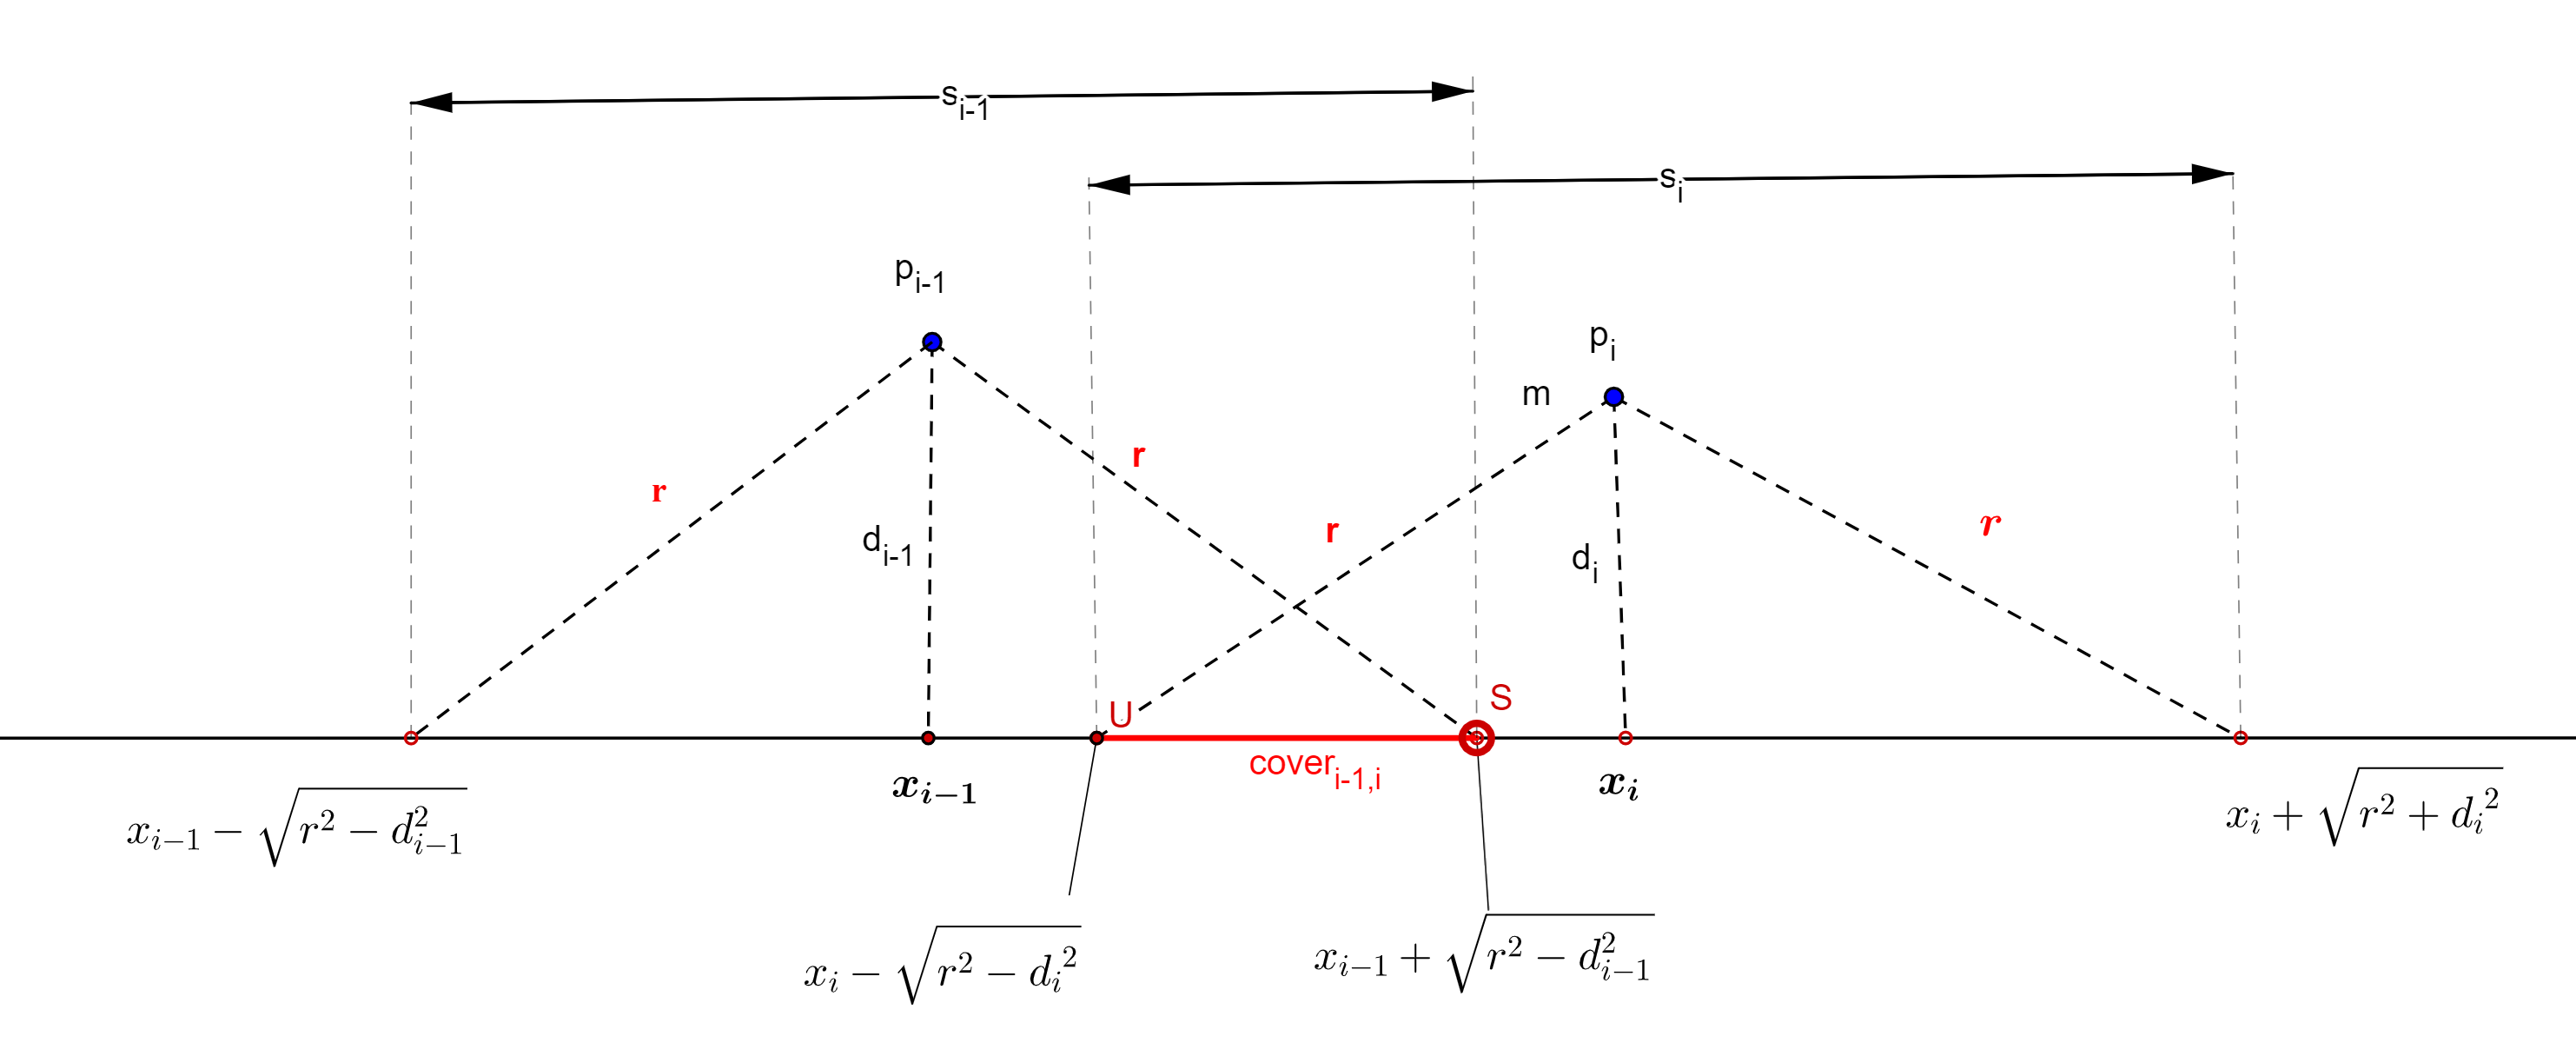
\includegraphics[scale=1.3]{images/geogebra-export (3).png}
\centering
\caption{Σχήμα 1}
\end{center}

\begin{center}
    \\
\end{center}
\textbf{Βελτιστότητα}\\
Βασική υπόθεση: Ο αλγόριθμός μας τοποθετεί έναν κύκλο για 1 σημείο. \\
Επαγωγική υπόθεση: Έστω ότι ο αλγόριθμος μας είναι βέλτιστος για n σημεία. \\
Για n-1 σημεία υπάρχουν 2 περιπτώσεις: \\
\textbf{1.} Το σημείο είναι στο εσωτερικό του τελευταίου κύκλου που έχουμε τοποθετήσει. Επομένως, δε χρειάζεται να τοποθετήσουμε νέο κύκλο και επιστρέφουμε το βέλτιστο αριθμό κύκλων. \\
\textbf{2.} Το σημείο είναι εκτός του τελευταίου κύκλου που έχουμε τοποθετήσει. Ο τελευταίος κύκλος που έχουμε τοποθετήσει , όπως και οι προηγούμενοι του, βάσει του αλγορίθμου μας είναι στη δεξιότερη δυνατή θέση ώστε να καλύπτουν το βέλτιστα τα n-1 σημεία και έτσι δε γίνεται να μετακινηθούν κάπως προκειμένου να καλύψουν το νέο σημείο. Έτσι προσθέτουμε με τον τρόπο που περιγράφει ο αλγόριθμος μας έναν νέο κύκλο. Επιστρέφεται πάλι λοιπόν ο βέλτιστος αριθμός κύκλων. \\
Έτσι αποδείξαμε ότι ο αλγόριθμός μας έιναι βέλτιστος.\\
\begin{center}
    \\
\end{center}
\textbf{Πολυπλοκότητα} \\
Η πολυπλοκότητα του άπληστου αλγορίθμου μας είναι ουσιαστικά O(nlogn + n) , nlogn για την ταξινόμηση και n για τη γραμμική τοποθέτηση των κύκλων έπειτα. Άρα τελικά είναι O(n\cdot logn)


\section*{Άσκηση 2: Μεταφορά Δεμάτων }
\subsection*{α.}
Στο πρώτο κομμάτι της άσκησης μας δίνονται ουσιαστικά 3 άπληστα κριτηρία που ενδεχομένως λύνουν το πρόβλημα της ασφαλούς στοίβαξης. \\
Άρχικά θα απορρίψουμε τα 2 πρώτα κριτήρια με τη χρήση ενός αντιπαραδείγματος για το καθένα:
\subsubsection*{1.} Έστω 2 πακέτα με $(w_{i},d_{i})$ τα εξής: (5,1) και (4,20). Με βάση το κριτήριο του βάρους η στοίβαξη θα είναι: 
\begin{center}
    (4,20) \\
    (5,1) 
\end{center}
Αυτή παρατηρούμε ότι είναι λανθασμένη αφού η αντοχή του κάτω πακέτου είναι μόνο 1,μικρότερη του βάρους 4 του από πάνω πακέτου. Η ασφαλής στοίβαξη για τα δύο κουτιά μπορούμε εύκολα να δούμε ότι είναι η αντίστροφη . 

\subsubsection*{2.} Με όμοιο τρόπο, έστω 2 πακέτα με $(w_{i},d_{i})$ τα εξής: (2,4) και (5,3). Με βάση το κριτήριο της αντοχής η στοίβαξη θα είναι :
\begin{center}
    (5,3) \\
    (2,4) 
\end{center}
Αυτή παρατηρούμε ότι είναι λανθασμένη αφού η αντοχή του κάτω πακέτου(4) είναι μικρότερη του βάρους του απο πάνω πακέτου(5). Εύκολα παρατηρούμε ότι με την αντίστροφη στοίβαξη των 2 πακέτων θα επιτυγχάναμε την ασφαλή τους στοίβαξη.

\subsubsection*{3.} 
Για το τρίτο κριτήριο θα αποδείξουμε την ορθότητα του. Δηλαδή ότι όταν υπάρχει τρόπος για να επιτευχθεί η ασφαλής στοίβαξη n πακέτων, το κριτήριο που στοιβάζει τα πακέτα με βάση το άθροισμα βάρους κι αντοχής, δηλαδή με $(w_{1}+d_{1})\ge (w_{2}+d_{2}) \ge... \ge (w_{n}+d_{n})$  επιτυγχάνει μία ασφαλή στοίβαξη. \\
Έστω μία βέλτιστη λύση, η οποία επιτυγχάνει την ασφαλή στοίβαξη n πακέτων. Ψάχνουμε να βρούμε στη στοίβαξη κοιτώντας από κάτω προς τα πάνω το πρώτο πακέτο-στοιχείο i για το οποίο δε θα ισχύει το κριτήριο 3.\\\\
 \textbf{1η Περίπτωση:} Αν δεν υπάρχει το i τότε το κριτήριό μας είναι ήδη βέλτιστο.\\\\
 \textbf{2η Περίπτωση:} Αν υπάρχει τότε θα υπάρχει και κάποιο στοιχείο j τοποθετημένο πιο πάνω από το i με $w_i + d_i < w_j + d_j$ (1). \\

Αυτό επόμενως θα σημαίνει τα 2 παρακάτω :
\begin{itemize}
    \item $d_j \ge \sum_{k=j+1}^{n} w_k \ $  (2)
    \item $d_i \ge \sum_{k=i+1}^{j-1} w_k \ + w_j + \sum_{k=j+1}^{n} w_k \ $  (3)
\end{itemize}
    
Άρα μέσω της (1) και της (3) έχω :
\begin{center}
$ w_i + \sum_{k=i+1}^{j-1} w_k \ + w_j + \sum_{k=j+1}^{n} w_k \ < w_j + d_j =>$ \\
$ w_i + \sum_{k=i+1}^{j-1} w_k \ + \sum_{k=j+1}^{n} w_k \ < d_j =>$
\\
$d_j \ge w_i + \sum_{k=i+1}^{j-1} w_k \ + \sum_{k=j+1}^{n} w_k$
\end{center}
Το παραπάνω μας δείχνει ότι το στοιχείο j έχει τέτοια αντοχή που μπορεί να αντέξει ουσιαστικά όλα τα πακέτα της στοίβας από το i και πάνω (το i, αυτά από το i μέχρι το j,και αυτά από το j και πάνω). Επομένως, το στοιχείο j μπορεί με ασφάλεια να μετακινηθεί κάτω από το i και έτσι να πληροί και αυτό το κριτήριο μας. Βέβαια πρέπει να αποδείξουμε ότι αυτη η μετακίνηση δε θα επηρεάσει κανένα από τα υπόλοιπα n πακέτα. \\
Για τα πακέτα από το j και πάνω δεν αλλάζει τίποτα. Για τα πακέτα από το i μέχρι το j μειώνεται το βάρος από πάνω τους αφού αφαιρείται το j.Ενώ για τα πακέτα 1 έως i επίσης δεν αλλάζει τίποτα αφού το βάρος από πάνω τους παραμένει ίδιο.\\
Έτσι αποδείξαμε και στις 2 περιπτώσεις ότι αν για n πακέτα υπάρχει ασφαλής στοίβαξη τότε με την παραπάνω μέθοδο θα υπάρχει και ασφαλής στοίβαξη με το κριτήριο μας.\\

\subsection*{β.}
Στο ερώτημα αυτό θέλω να βρω τη στοίβαξη που μεγιστοποιεί το κέρδος. Παρατηρούμε, πως το πρόβλημα μας μοιάζει με το knapsack problem. Ωστόσο την περίπτωση μας κάθε φορά που προσθέτουμε ένα αντικείμενο στη στοίβα αλλάζει η αντοχή της στοίβας - ή αντίστοιχα αλλάζει η "χωρητικότητα" του knapsack μας. 
Θα χρησιμοποίησουμε δυναμικό προγραμματισμό και ο αλγόριθμός μας θα έχει ως εξής.
\begin{itemize}
    \item Αρχικά εκμεταλλεύομενει το άπληστο κριτήριο του (α3) ταξινομούμε τα n πακέτα με βάση το άθροισμα $w_i+d_i , i=1,2...n$ .
    \item Έπειτα θα χρησιμοποίησουμε έναν πίνακα μεγέθους n x $d_max + 1$ όπου $d_max$ είναι η μέγιστη αντοχή που παρατηρείται στα n πακέτα. Έστω P ο πίνακας αυτός. Στή θέση P[i][d] θα βρίσκεται το μέγιστο κέρδος που μπορώ να έχω με τα πρώτα i πακέτα με μία στοίβαξη αντοχής d. Η στήλη $d_{max}$ του πίνακα, ουσιαστικά προσομοιώνει το έδαφος δηλαδή μία αντοχή ίση με $\infty$ πάνω στην οποία θα τοποθετήσουμε το 1ο πακέτο.
    \item Δημιουργούμε λοιπόν την εξής αναδρομική σχέση : \\
    \begin{equation*}
    P(i,d)=\begin{cases}
          0 \quad &\text{αν} \, $i=0 ή d=0$ \\
          P(i-1 , d) \quad &\text{αν} \, $w_i > d$ \\
          $max$\ \{$P(i-1 , d) , P(i-1 , d_{min}) + p_i$\} \quad &\text{αν} \, $w_i \le d $
     \end{cases}
   \end{equation*} 
   ,όπου $d_{min}$ = min\{ d-$w_i$ , $d_i$\} ,δηλαδή ότι κάθε φορά που προσθέτουμε ένα νέο αντικείμενο i , η νέα αντοχή είναι η μικρότερη μεταξύ της προηγούμενης αντοχής μείον το $w_i$ ή της αντοχής $d_i$.
   \item Για τη λύση του προβλήματος πηγαίνω στη θέση P[n][$d_{max}+1$] όπου θα βρίσκεται το μέγιστο κέρδος για n πακέτα που τοποθετούνται αρχικά με περιορισμό άπειρης αντοχής($d_{max}+1$ ),δηλαδή του δαπέδου. 
\end{itemize} 

\begin{center}
    \\
\end{center}
\textbf{Επεξήγηση και Ορθότητα} \\
Για να βρω κάθε φορά το μέγιστο κέρδος για i πακέτα και μία αντοχή d, ελέγχω ουσιαστικά αν μπορώ να τοποθετήσω το i-οστο στοιχείο "πάνω" στην αντοχή d (d \ge $w_i$ ). Αν γίνεται ελέγχω από τι λαμβάνω μεγαλύτερο κέρδος:
\begin{enumerate}
    \item Να το συμπεριλάβω στη λύση μου , δηλαδή να βάλω από πάνω από την αντοχή $d_{min}$ i-1 πακέτα και να πάρω κέρδος $p_i$ + P(i-1,$d_{min}$)\\
    ή 
    \item Να μην το συμπεριλάβω στη λύση μου και να πάρω κέρδος από τα i-1 πακέτα που μένουν.
\end{enumerate} 
Η ορθότητα του αλγορίθμου αποδεικνύεται από την αρχή της βελτιστότητας. Δηλαδή η τελική λύση προέρχεται από βέλτιστες λύσεις στα υποπροβλήματα που προκύπτουν. Λύνουμε τα προβλήματα αναδρομικά, δηλαδή έχουμε i πακέτα κάθε φορά που μειώνονται με βήμα 1 ,όπου $i \le n$, και παίρνω τελικά τη βέλτιστη λύση για πλήθος n πακέτων .\\\\
\textbf{Πολυπλοκότητα} \\
Έχουμε έναν πίνακα μεγέθους n x ($d_{max}+1$ όπου κάθε κελί του απαιτεί χρόνο Ο(1) για να συμπληρωθεί. Άρα ,ομοίως με το knapsack problem έχουμε συνολικά χρονική πολυπλοκότητα Ο(n\cdot $d_{max}$ ) . \\

\section*{Άσκηση 3: Τριγωνοποίηση Πολυγώνου}

Για τη λύση του προβλήματος της τριγωνοποίησης του πολυγώνου θα θεωρήσουμε για τη συνέχεια τους εξής συμβολισμούς:
\begin{itemize}
    \item $Δ(u_iu_ju_k)$ το άθροισμα των πλευρών ενός τριγώνου με κορυφές τις $u_i,u_j,u_k$ (με βάση την εκφώνηση της άσκησης)
    \item c[i][k] το ελάχιστο κόστος τριγωνοποίησης του πολυγώνου με κορυφές $u_iu_{i+1}...u_k$
\end{itemize} Για την δόμηση του αλγορίθμου μας θα ακολούθησουμε τα εξής βήματα:
\begin{itemize}
    \item Έστω c[0][n-1] το κόστος της ελάχιστης τριγωνοποίησης για ένα πολύγωνο n κορυφών. Ένα πολύγωνο από το σημείο i έως το σημείο k περιέχει 2 επιμέρους πολύγωνα για ένα σημείο j με $i<j<k$, με ελάχιστα κόστη c[i][j] και c[j][k] αντίστοιχα. Εδώ υπάρχουν 2 περιπτώσεις: 1. να ισχύει $k<i+2$ ,δηλαδή να έχουμε λιγότερες από 3 κορυφές ,όπου δεν υπάρχουν επιμέρους πολύγωνα και 2. ισχύει $ k \ge i+2 $, δηλαδή για n-γωνα με $n \ge 3$ όπου υπάρχει μία ή περισσότερες τριγωνοποιήσεις. Έτσι χτίζουμε την παρακάτω αναδρομική σχέση :
    \item \begin{equation*}
    c[i][k]=\begin{cases}
          0 \quad &\text{αν} \, k< $ i + 2$ \\
          $min_{i<j<k}$\ \{$c[i][j] + c[j][k] + Δ(u_iu_ju_k)$\} \quad &\text{αν} \, $k \ge i + 2 $
     \end{cases}
\end{equation*}
    \item Ταυτόχρονα καταγράφω σε πίνακα m[n x n] το j στη θέση m[i][k]. Αυτό θα με βοηθήσει να λύσω το πρόβλημα με αναδρομή με απομνημόνευση.

\end{itemize}

Στο σημείο αυτό, κάνοντας μία παρένθεση, παρατηρούμε πως μέχρι στιγμής η δόμηση της λύσης για το πρόβλημα της τριγωνοποίησης πολυγώνων "θυμίζει" τον Αλυσιδωτό Πολλαπλασιασμό Πινάκων που μελετήθηκε και στις διαλέξεις του μαθήματος. Μπορούμε μάλιστα να κάνουμε μία 1-προς-1 αντιστοίχιση των 2 προβλήματων αν σκεφτούμε πως: \\
1. Tο c[i][k] είναι το ελάχιστο κόστος πολλαπλασιασμού πινάκων A[$d_i x d_j$] x A[$d_j x d_k$]\\ 
2. Tα c[i][j] και c[j][k] είναι τα αντίστοιχα κόστη για τους επί μέρους πολλαπλασιασμούς \\ 
3. Tο $Δ(u_iu_ju_k)$ είναι το κόστος του πολλαπλασιασμούς πινάκων $(d_i  x d_j)x(d_j x d_k)$ .\\ 

\begin{itemize}
    \item Συνεχίζοντας, θα διαμορφώσουμε τη λύση ως εξής. Γνωρίζοντας πως στη θέση m[0][n-1] βρίσκεται το $j_0$ ξέρω ότι το $Δ(u_0u_{j_0}u_n)$ είναι μέρος μίας ελάχιστης τριγωνοποίησης. Βρίσκω περισσότερα τρίγωνα με προσπέλαση των m[0][$j_0$] και m[$j_0$][n-1] και κάθε φορά προσθέτω στο συνολικό άθροισμα το αντίστοιχο $Δ(u_iu_ju_k)$ που βρίσκω. Συνεχίζω, μέχρι να βρω όλα τα τρίγωνα της ελάχιστης τριγωνοποίησης.
\end{itemize}

\textbf{Πολυπλοκότητα} 
Η λύση του προβλήματος μας απαιτεί χώρο Ο($n^2$) , λόγω των 2 πινάκων m και c μεγέθους (nxn). Επίσης έχει χρονική πολυπλοκότητα O($n^3$) αφού κάνει ουσιαστικά n πράξεις για $n^2/2$ στοιχεία (τα μισά του πίνακα c(n x n) ). \\

\newpage
\section*{Άσκηση 4: Τοποθέτηση στεγάστρων (και Κυρτό Κάλυμμα)}
\subsection*{α.}

Για τη λύση μας σε αυτό το πρόβλημα θα χρησιμοποιήσουμε δυναμικό προγραμματισμό. Για την αρχή της βελτιστότητας , έστω ότι για να καλύψουμε βέλτιστα τα σημεία 0$<x_1<x_2<...<x_n<L$ χωρίζουμε το πρόβλημα σε 2 υποπροβλήματα για τα σημεία $x_1<...<x_j$ και $χ_{j+1}<...<x_n$ αντίστοιχα,όπου $1 \le j \le n$. Το ελάχιστο κόστος τοποθέτησης στεγάστρων για τα σημεία μας θα προκύψει από τον υπολογισμό του αντίστοιχου ελάχιστου κόστους για κάθε ένα από τα υποπροβλήματα ή την τοποθέτηση εν΄ςο ενιαίου στέγαστρου από το $x_1$ έως to $x_n$ αναλόγως με το ποια επιλογή έχει μικρότερο κόστος. \par
Έστω τώρα cost[i][k] , $1 \le i \le n$ , $1 \le k \le n$ το ελάχιστο κόστος για τη στέγαση από το σημείο $x_i$ έως το σημείο $x_k$. Με βάση την εκφώνηση, η στέγαση ενός σημείου αποκλειστικά έχει κόστος C και άρα cost[1][1] = C. Αντίστοιχα, η στέγαση από ένα σημείο a σε ένα σημείο b έχει κόστος $(a-b)^2 + C$. Επομένως με βάση τα παραπάνω καταλήγουμε στην κατασκευή της παρακάτω αναδρομικής συνάρτησης:
\begin{itemize}
    \item\begin{equation*}
    cost[i][k]=\begin{cases}
          C \quad &\text{αν} \, $ i=k$ \\
          $min_{i\le j<k}$\ \{$cost[i][j] + cost[j+1][k]  ,  (x_k - x_i)^2 + C) $ \} \quad &\text{αν} \, $ i \ne k $
        \end{cases}
    \end{equation*}
\end{itemize}

Για τη λύση του προβλήματος μέσω της αναδρομικής συνάρτησης θα λειτουργήσουμε ως εξής. Θέλουμε να βρούμε ουσιαστικά την τιμή cost[1][n]. Aυτόματα το πρόβλημα μας σπάει σε 2 , τα οποία λύνουμε μέσω της αναδρομικής συνάρτησης. Συνεχίζουμε μέχρι να φτάσουμε σε αποτέλeσμα που δεν απαιτεί επιπλέον κλήσεις της αναδρομικής συνάρτησης. Η χρονική πολυπλοκότητα της παραπάνω επίλυσης είναι O($n^3$) ομοίως και με την άσκηση 3. Αφού εκτελούμε n πράξεις για $n^2/2$ στοιχεία. 


\newpage
\section*{Άσκηση 5: Καλύπτοντας ένα δέντρο}
\subsection*{α.}
Για το πρόβλημα θα ακολουθήσουμε τα εξής βήματα. \\
\textbf{Βήμα 1:} Θα δημιουργήσουμε έναν πίνακα διαστάσεων n x n στον οποίο θα αποθηκεύουμε την απόσταση μεταξύ 2 οποιονδήποτε κόμβων, δηλαδή πως θα επηρεάσει ένας κόμβος όλους τους άλλους αν είσαχθει στο Κ. Για την κατασκευή του πίνακα αυτού κάνουμε την παραδοχή ότι οι κόμβοι είναι αριθμημένοι από 0 έως n-1 με βάση τα επίπεδα που βρίσκονται. Για παράδειγμα, όπως στο δέντρο που φαίνεται παρακάτω. 

\begin{center}
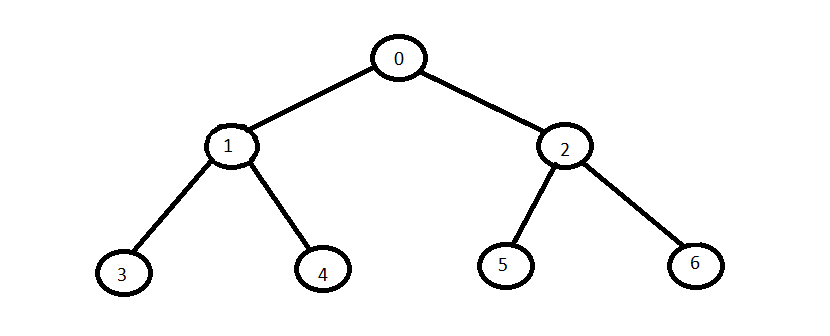
\includegraphics[scale=0.8]{images/tree.png}
\centering
\end{center}

Έτσι, προκυπτεί η εξής αναδρομική σχέση με την οποία γεμίζουμε τον πίνακα μας , έστω dist[i][j]:

    \begin{equation*}
    dist[i][k]=\begin{cases}
          0 \quad &\text{αν είναι leaf και} \, $ i=j$ \\
          -1 \quad &\text{αν είναι leaf και} \,  i \ne j \\
          $min$\ \{$dist[r\_sub][j]+1 , dist[l\_sub][j]+1$ \} \quad &\text{αν κάποιο από τα 2 είναι -1 το προσπερνώ} \, \\
          -1 \quad &\text{αλλιώς} \
        \end{cases}
    \end{equation*}

Τρέχω άλλη μία φορά τον πίνακα και βάζω όπου έχω -1 το dist[root][j]. \\

\textbf{Βήμα 2:} Έπειτα, θέλω να διαλέξω κ κόμβους ώστε να είναι βέλτιστοι ως προς το ελάχιστο κόστος. Θα σκεφτώ ως εξής. 
\begin{itemize}
    \item Διαλέγω το ελάχιστο από τα μέγιστα κόστη κάθε γραμμης.
    \item Αν υπάρξουν 2 ίσα κόστη, επιλέγω εκείνο με το ελάχιστο άθροισμα στοιχείων γραμμής.
\end{itemize}

\textbf{Βήμα 3:} Στη συνέχεια ενημερώνω τον πίνακα dist ως εξής. Έστω ότι έχω τοποθετήσει τα στοιχεία που έχω διαλέξει έως τη δεδομένη στιγμή σε έναν 1D πίνακα έστω pith[i],i=0,1...k. Ενημερώνω τον πίνακα dist με την μέθοδο: \\
\begin{center}
    dist[i][j] = max\{ dist[i][j] , dist[pith[i]][j]\}
\end{center}

Επαναλαμβάνω το βήμα 2 k φορές. 
Τελειώνω βρίσκοντας το max στοιχείο του dist και αυτό θα είναι το ελάχιστο κόστος.

\textbf{Πολυπλοκότητα} \\
Η κατασκευή του πίνακα έχει πολυπλοκότητα O($n^2$). Επαναλαμβάνω το βήμα 2 Ο(k) φορές  και το βήμα 3 επίσης Ο(k) φορές (πίνακας μεγέθους k).\\
Συνολικά λοιπόν έχω πολυπλοκότητα O($n^2k^2$).

\subsection*{β.}
Για την απάντηση του ερωτήματος αυτού θα υλοποιήσουμε έναν άπληστο αλγόριθμο ο οποίος βρίσκει κάθε φορά τον κόμβο με το μεγαλύτερο cost(K), έστω u, και επιλέγει για το υποσύνολο K τον πρόγονο του με απόσταση z. Ουσιαστικά , ο αλγόριθμος μας θα τρέχει επαναληπτικά μέχρι να μην υπάρχει κόμβος με κόστος μεγαλύτερο του z.\par

Η ορθότητα του αλγορίθμου βασίζεται στο επιχείρημα ανταλλαγής στρατηγικής. \\
Για τον κόμβο u στον οποίο αναφερθήκαμε   παραπάνω πρέπει αναγκαστικά να ικανοποιηθεί η συνθήκη
$cost(T) < z$ αφού είναι εκείνος με το μεγαλύτερο cost(T). Εάν επιλέξουμε οποιονδήποτε άλλο κόμβο για το Κ εκτός από τον πιο μακρινό ικανό πρόγονο του,δηλαδή εκείνον σε απόσταση z, τότε δε θα μεγιστοποιήσουμε τον αριθμό των κόμβων για τους οποίους η συνθήκη ικανοποιείται με μία επανάληψη. \par
Η υλοποίηση του αλγορίθμου μπορεί να γίνει με μία DFS διάσχιση η οποία κάθε φορά που "μαρκάρει" έναν κόμβο ως visited θα επιστρέφει και το μέγιστο ύψος των παιδιών του . Όταν ένας κόμβος λάβει από κάποιο παιδί του την τιμή z ως ύψος , τότε πρέπει να επιλαγεί για το Κ και να επιστρέψει στον δικό του πατέρα το νέο του ύψος δηλαδή 1 (αφού θα ανήκει στο Κ πλέον ο κόμβος αυτός ). Τέλος, αν με το πέρας του αλγορίθμου δεν έχει επιλεγεί η ρίζα , επιλέγουμε κι εκείνη. Η πολυπλοκότητα του αλγορίθμου αυτού είναι O($n + e$) ,δηλαδή λόγω binary tree Ο(n). \par
Για την επίλυση του ερωτήματος (α) θα κάνουμε δυαδική αναζήτηση μεταξυ του 0 και του n για να βρούμε το μικρότερο z που απαιτεί k κόμβους. Η χρονική πολυπλοκότητα γι'αυτό θα είναι Ο($nlogn$) αφού στη χειρότερη περίπτωση ο παραπάνω αλγόριθμος θα εκτελεστεί logn φορές. 

\end{document}
